\documentclass[11pt]{amsart}
%\documentclass[11pt]{report}
\usepackage[toc,page]{appendix}
\usepackage{float}
\usepackage{mathtools}
\usepackage{geometry}        % See geometry.pdf to learn the layout options.
\geometry{a4paper}           % ... or a4paper or a5paper or ...
%\geometry{landscape}        % Activate for for rotated page geometry
%\usepackage[parfill]{parskip} % Activate to begin paragraphs with empty line
\usepackage{graphicx}
\usepackage{amssymb}
\usepackage{epstopdf}

\usepackage[most]{tcolorbox}
\definecolor{block-gray}{gray}{0.85}
\newtcolorbox{myquote}{colback=block-gray,grow to right by=+0mm,grow to left by=-10mm, boxrule=0pt,boxsep=0pt,breakable}

\DeclareGraphicsRule{.tif}{png}{.png}{`convert #1 `dirname #1`/`basename #1 .tif`.png}
\graphicspath{ {images/} }

\renewcommand{\familydefault}{\sfdefault}
\newcounter{defctr}

\title{Parsing Expression Grammar Assembly}
\author{Kees-Jan Hermans}
%\date{}                     % Activate to display a given date or no date

\begin{document}
\maketitle

\textbf{Abstract}

Because of its complexity - nested binary TLV encoding and various
compression schemes -
parsing BER and BER-like formatted messages (such as X.509 certificates or
SNMP messages) is considered problematic. To my
knowledge, formal parsing of BER is not
addressed by available solutions. Instead, custom, hand
coded solutions or generated code prevail. This is a security risk from a
point of view of bugs or code proliferation. The changes proposed in the
paper extend Parsing Expression Grammar
(PEG), which is an unambiguous, top-down, recursive descent parsing algorithm.
This PEG extension enables it to parse BER formats, while retaining a
simple grammar definition, and requiring only minimal changes to the
resulting assembly and bytecode interpreter. This paper also shows that,
having implemented those changes, and using a grammar that closely mimics
its ASN.1 counterpart definition, it is possible to split up X.509 and SNMPv3
messages in their underlying parts. Other findings presented
are that this extension allows BER well-formedness checks, as well as ASN.1
definition checks, and that it allows content, such as digital
signatures, to be isolated (captured) from the input (allowing for a subsequent
cryptographic content integrity check). It shows how OIDs
can be broken up in their composing parts, and the way in which text
fields of binary formats can be text-parsed (\textit{eg} email address
validation). Further study is required with respect to potential machine
implementations of the PEG engine, and the representation of binary
fields such as INTEGERs and OIDs from the input capture list.


\vspace*{3\baselineskip}

%\begin{figure}[H]
%\centering
%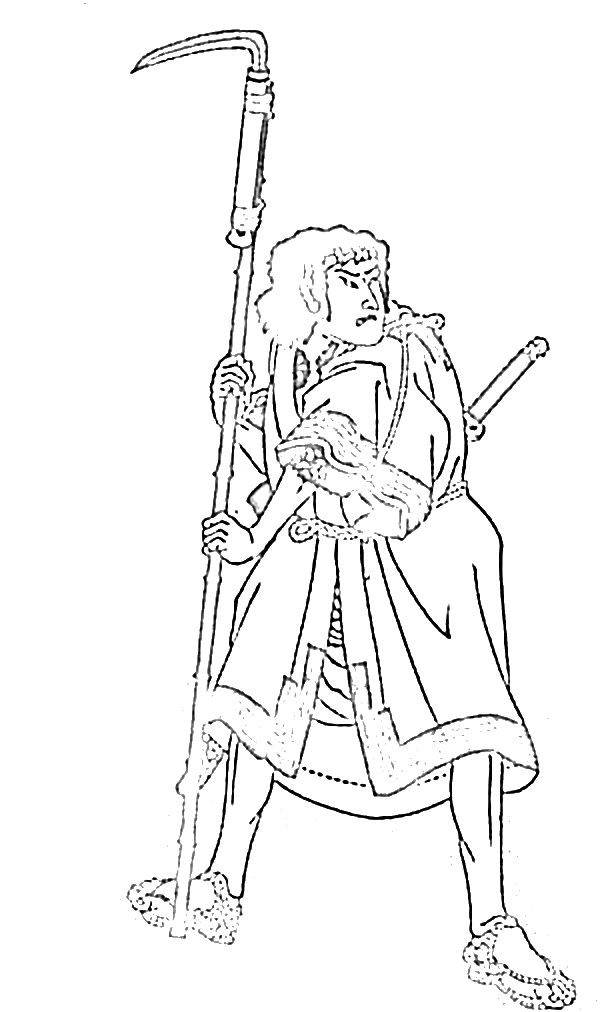
\includegraphics[width=60mm]{naigama}
%\end{figure}

\vfill

\begin{table}[]
\centering
\begin{tabular}{ll}
Accompanies release & \input{../../../release} \\
Author &  Kees-Jan Hermans / kees.jan.hermans@gmail.com \\
Classification & - \\
Generated on & \today \\
\end{tabular}
\end{table}

\newpage

\tableofcontents

\setlength{\parindent}{4em}
\setlength{\parskip}{1em}

\newpage

\section{Rationale}

In the whitepapers of Ierusalemschi et al \cite{bib:peg}
on Parsing Expression Grammars,
an assembly language is proposed that grammar is
compiled to, transforming a potentially infinitely deep structure
description into a list of instructions, allowing a simple state machine
with an endless loop to execute what would otherwise require 
ecursion in the execution of the parser.

It's a simple, elegant, efficient and secure concept:
with somewhere around 20 instructions, one can
formulate all conditions that a (text) parser could encounter
to a relatively deep level of syntactic understanding (even down
to such things as dynamically matching open- and closing XML tags,
for example).

This assembly language's instructions however,
oftentimes perform a combination of underlying manipulations of the
state machine, of which many make a repeated appearance.
For example, the \texttt{commit $<$label$>$} instruction is assumed to
perform the following steps:

\begin{itemize}
\item Pop a 'choice' element off the stack (must be the top element).
\item Jump to $<$label$>$
\end{itemize}

Where the \texttt{FAIL} condition (and the \texttt{fail} instruction)
is assumed to:

\begin{itemize}
\item Pop any item that isn't a 'choice' element off the stack.
\item Pop a 'choice' element off the stack (must now be the top element).
\item Recreate the machine state stored in that element.
\item Jump to the offset stored in that element.
\end{itemize}

And the \texttt{partialcommit $<$label$>$} instruction is assumed to
 \footnote{The expansion of the 'partialcommit' instruction has been purposely
worded in a convoluted manner; the original paper means the 'partialcommit'
as an optimization, where the 'choice' element on the stack isn't popped
and subsequently pushed, but \textit{updated}. In this paper, I propose
a different model of stack, that allows for efficient popping and pushing.}
:

\begin{itemize}
\item Pop a 'choice' element off the stack (must be the top element).
\item Update the input position in the machine state stored in that element.
\item Push the 'choice' element back on the stack.
\item Jump to $<$label$>$
\end{itemize}

However, if we look at the way all these instructions are conceptualised,
we can see a lot of similarities: the stack is pushed onto, and popped from,
the input position is guarded and increased, and there are jumps.
These should all be familiar to people who know 'proper' assembly
languages such as i386 or ARM. Note that the goal of this paper is not
to promote compiling down to an \textit{actual} assembly language, but
rather to one that is still abstract, but has more similarities with
those assembly languages.

Wouldn't it be worth exploring, then,
if the 'sub instructions' were somehow made more concrete, and actually
compile a PEG not to the whitepaper's assembly language, but to one that
is more elementary? Let's explore the arguments as to why this could be so.
That is to say: why pursuing another, 'deeper' assembly for PEG's could be
beneficial.

\begin{itemize}
\item For one, 'deeper', more 'CPU like' assembly instructions can be monitored
more ...
\item There could be (even) fewer of them.
\item And it could yield faster and / or yield better optimizations and
thereafter be faster.
\item Hardware implementations of the machine could be easier to implement.
\end{itemize}

The obvious downsides, from a first glance, would be:
The bytecode would be bigger; the original bytecode is also a means to
compress functional logic. The upside to that is that the machine size
would be smaller.
More elementary instructions also lack security, because they lack more
context in which their monitoring could take place.
Forensics, trying to discover why a piece of grammar would yield a
certain piece of bytecode, would be more difficult.

\section{Instructions}

\subsection{The FAIL Region}

\subsection{The Stack}

\subsection{Instruction Breakdown}

\subsubsection{Any}

\begin{itemize}
\item Set the failure region to 'JUMP FAIL'
\item Is the input pointer less than the input length (otherwise FAIL)?
\item Move the input pointer one up
\end{itemize}

\subsubsection{Char n}

\begin{itemize}
\item Set the failure region to 'JUMP FAIL'
\item Is the input pointer less than the input length (otherwise FAIL)?
\item Is the input character equal to \textit{n} (otherwise FAIL)?
\item Move the input pointer one up
\end{itemize}

\subsubsection{Span $<$set$>$}

\subsubsection{Set $<$set$>$}

\subsubsection{Jump $<$label$>$}

\begin{itemize}
\item As is, this instruction won't be broken down any further.
\end{itemize}

\subsubsection{Choice $<$label$>$}

\begin{itemize}
\item Push the input pointer
\item Push the action list length
\item Push the resolved address from $<$label$>$
\item Push a stack element type signifier (if you want a stack guard)
\end{itemize}

\subsubsection{Call $<$label$>$}

\begin{itemize}
\item Push the return address (the address of this instruction + its length)
\item Push a stack element type signifier (if you want a stack guard)
\end{itemize}

\subsubsection{Return}

\begin{itemize}
\item Pop a stack element (if you guard your stack, this must be of type 'Call')
\item Pop an address
\item Jump to the address
\end{itemize}

\subsubsection{Commit $<$label$>$}

\begin{itemize}
\item Pop a 'choice' element off the stack (must be the top element).
\item Pop and discard
\item Pop and discard
\item Pop and discard
\item Jump to $<$label$>$
\end{itemize}

\subsubsection{Fail}

\begin{itemize}
\item Jump to the special 'FAIL' label
\end{itemize}

\subsubsection{Failtwice}

\subsubsection{Partialcommit}

\subsubsection{Backcommit}

\section{Assembly}
\label{sec:assembly}

A Naigama assembly file or buffer consists of sequences of
whitespace, comments, labels, and (parametrized) instructions, separated
by new lines, and denoted in ASCII text.

Naigama assembly is taken by the Naigama assembler program (naia) and turned
into bytecode.

\begin{myquote}
\begin{verbatim}
-- Compilation of: TEST <- { 'a' } { 'a' } { 'a' / 'b' }

  call TEST
  end
-- Rule
TEST:
  opencapture 0
  char 61
  closecapture 0 0
  opencapture 1
  char 61
  closecapture 1 0
  opencapture 2
  catch __LABEL_30 -- alternative
  char 61
  commit __LABEL_31
__LABEL_30:
  char 62
__LABEL_31:
  closecapture 2 0
  ret

\end{verbatim}
\end{myquote}
\textit{Example of a piece of Naigama assembly}

\subsection{Comments}

Just like in Naigama grammar,
comments in Naigama assembly start with two minus signs, and end at
a new line. They can be given on separate lines, or they can be
postfixed to instructions or labels.

\subsection{Labels}

Labels are identifiers (the same identifiers as in their definition
in the grammar chapter) or numbers, followed by a colon sign. They are used
as positions for the bytecode to jump to, when used by instructions.

When performing the assembly, the Naigama assembler program resolves
each label to their offset in the resultant bytecode, and replaces each
reference to a label with that offset.

Labels don't quite disappear though - you have the option to make the
assembler program emit a so called 'labelmap' file, which stores the old
label names, mapped to the bytecode offsets given by the assembler,
and which can be used later
for debugging purposes by the bytecode execution engine.

When disassembling (bytecode to assembly), each instruction is always
prefixed by a label in the form of the instruction's offset in decimal,
so that jumps are always correct (but non descriptive).

\subsection{Instructions}


%\begin{table}[]
\begin{center}
\caption{Naigama Assembly Instructions}
\label{tab:naig_assembly}
\begin{longtable}{lll}
\textbf{Mnemonic} & \textbf{Param1} & \textbf{Param2} \\
\endhead
'any' &  &  \\
'backcommit' &  & LABEL \\
'call' &  & LABEL \\
'catch' &  & LABEL \\
'char' & char &  \\
'closecapture' & slot &  \\
'commit' &  & LABEL \\
'condjump' & register & LABEL \\
'counter' & register & value \\
'end' & code &  \\
'endisolate' &  &  \\
'endreplace' &  &  \\
'fail' &  &  \\
'failtwice' &  &  \\
'intrpcapture' &  &  \\
'isolate' & slot &  \\
'jump' &  & LABEL \\
'maskedchar' & char & mask \\
'noop' &  &  \\
'opencapture' & slot &  \\
'partialcommit' &  & LABEL \\
'quad' & quad &  \\
'range' & from & until \\
'replace' & slot & LABEL \\
'ret' &  &  \\
'set' & set &  \\
'skip' & number &  \\
'span' & set &  \\
'testany' &  & LABEL \\
'testchar' & char & LABEL \\
'testquad' & quad & LABEL \\
'testset' & set & LABEL \\
'trap' &  &  \\
'var' & slot &  \\
\end{longtable}
\end{center}
%\end{table}


See table [\ref{tab:naig_assembly}].

\subsection{Parameters}

Parameters follow the instruction in assembly text. They are separated
from the instruction and any other parameters by spaces. The following
types of parameters exist:

\subsubsection{Characters}

Character parameters are denoted as two byte hexadecimal values.

\subsubsection{Quads}

Quad parameters are denoted as eight byte hexadecimal values.

\subsubsection{Sets}

Set parameters are denoted as 64 byte hexadecimal values, representing
a bitmask of 256 possible booleans.

\subsubsection{Registers, Slots, Codes and Numbers}

These parameters are all denoted as decimal numbers.



\newpage
\section{Colofon}

\listoftables

\newpage

\begin{thebibliography}{12}

\bibitem{bib:peg}
  A Text Pattern-Matching Tool based on Parsing Expression Grammars
  https://www.inf.puc-rio.br/\textasciitilde roberto/docs/peg.pdf

\bibitem{bib:regex}
  Regular Expressions
  https://en.wikipedia.org/wiki/Regular\_expression

\bibitem{bib:backusnaur}
  Backus Naur Form
  https://en.wikipedia.org/wiki/Backus-Naur\_form

\bibitem{bib:yacc}
  Yacc Yet Another Compiler Compiler
  https://en.wikipedia.org/wiki/Yacc

\bibitem{bib:javascript}
  JavaScript, or ECMAScript
  https://www.ecma-international.org/publications/standards/Ecma-262.htm

\bibitem{bib:json}
  JSON, JavaScript Object Notation
  https://www.json.org/

\bibitem{bib:perl}
  Perl, the Perl Programming Language
  https://www.perl.org/

\end{thebibliography}


\end{document}
